\documentclass[tikz,border=5mm]{standalone}
\usepackage{pgfplots}
\usepackage{amsmath}
\pgfplotsset{compat=1.18}

% Explicit RGB color definitions
\definecolor{innerteal}{RGB}{0, 130, 130}
\definecolor{outerblue}{RGB}{0, 0, 128}
\definecolor{tangentred}{RGB}{204, 24, 66}
\definecolor{radiigray}{RGB}{100, 100, 100}
\definecolor{opdotted}{RGB}{80, 0, 80}

\begin{document}
	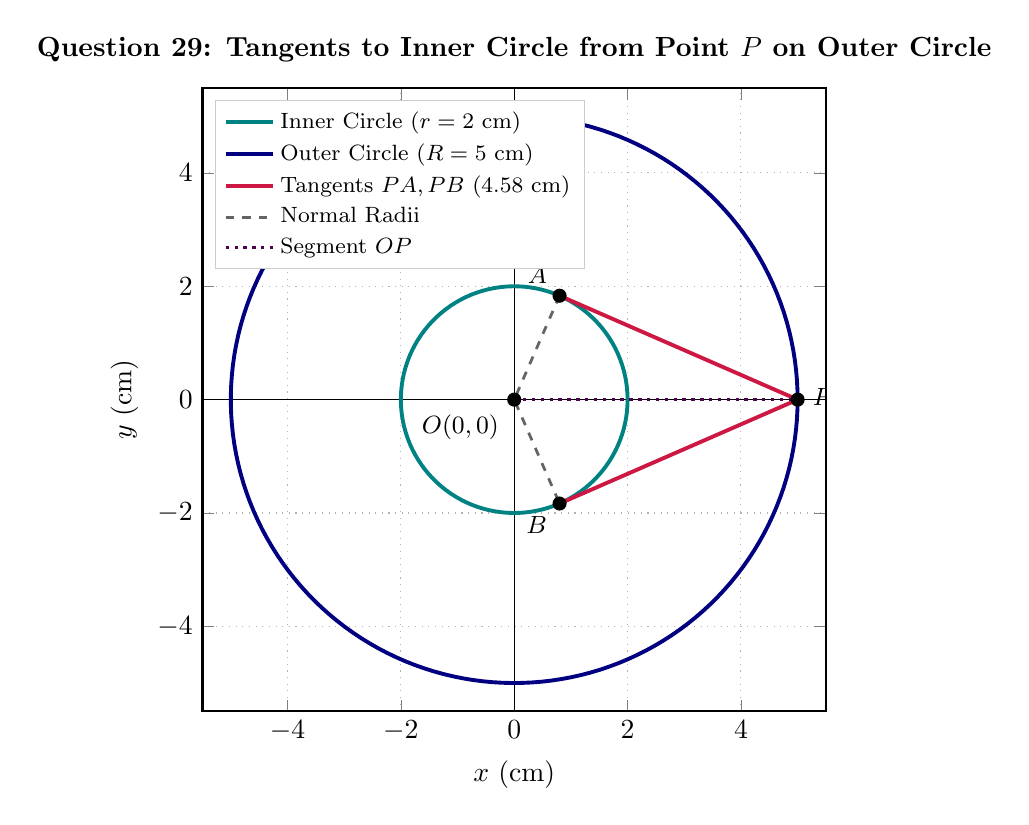
\begin{tikzpicture}
		\begin{axis}[
			width=9.5cm, height=9.5cm,
			title={\textbf{Question 29: Tangents to Inner Circle from Point $P$ on Outer Circle}},
			xlabel={$x\text{ (cm)}$}, ylabel={$y\text{ (cm)}$},
			xmin=-5.5, xmax=5.5,
			ymin=-5.5, ymax=5.5,
			xtick={-4,-2,0,2,4},
			ytick={-4,-2,0,2,4},
			axis equal image,
			grid=both,
			grid style={dotted, gray!60},
			axis line style={black, thick},
			legend cell align={left},
			legend style={at={(0.02,0.98)}, anchor=north west, font=\footnotesize, draw=gray!40}
			]
			% Origin axis lines
			\draw[black, thin] (axis cs:0,-5.5) -- (axis cs:0,5.5);
			\draw[black, thin] (axis cs:-5.5,0) -- (axis cs:5.5,0);
			
			% Inner Circle (r = 2)
			\addplot[innerteal, line width=1.4pt, domain=0:360, samples=120] ({2*cos(x)}, {2*sin(x)});
			\addlegendentry{Inner Circle ($r = 2\text{ cm}$)}
			
			% Outer Circle (R = 5)
			\addplot[outerblue, line width=1.4pt, domain=0:360, samples=180] ({5*cos(x)}, {5*sin(x)});
			\addlegendentry{Outer Circle ($R = 5\text{ cm}$)}
			
			% Tangents PA and PB: A = (0.8, 1.833), B = (0.8, -1.833), P = (5, 0)
			\addplot[tangentred, line width=1.4pt] coordinates {(0.8, 1.8330) (5, 0) (0.8, -1.8330)};
			\addlegendentry{Tangents $PA, PB$ ($4.58\text{ cm}$)}
			
			% Normal Radii OA and OB
			\addplot[radiigray, dashed, line width=1pt] coordinates {(0.8, 1.8330) (0, 0) (0.8, -1.8330)};
			\addlegendentry{Normal Radii}
			
			% Segment OP
			\addplot[opdotted, dotted, line width=1.2pt] coordinates {(0, 0) (5, 0)};
			\addlegendentry{Segment $OP$}
			
			% Points
			\node[circle, fill=black, inner sep=1.8pt] at (axis cs:0,0) {};
			\node[below left=2pt, font=\small] at (axis cs:0,0) {$O(0, 0)$};
			
			\node[circle, fill=black, inner sep=1.8pt] at (axis cs:5,0) {};
			\node[right=2pt, font=\small] at (axis cs:5,0) {$P(5, 0)$};
			
			\node[circle, fill=black, inner sep=1.8pt] at (axis cs:0.8, 1.8330) {};
			\node[above left=1pt, font=\small] at (axis cs:0.8, 1.8330) {$A$};
			
			\node[circle, fill=black, inner sep=1.8pt] at (axis cs:0.8, -1.8330) {};
			\node[below left=1pt, font=\small] at (axis cs:0.8, -1.8330) {$B$};
		\end{axis}
	\end{tikzpicture}
\end{document}